% 2023
% Unidad 06
% VOR



\subsection{Un poco de historia....}
\label{sec:06.VOR.historia}

% \begin{wrapfigure}{r}{0.35\textwidth} \centering
%   \includegraphics[keepaspectratio,width=0.3\textwidth]{06.radionavegacion/Imagenes/06.02.vor.imagenes/Marconi.eps}\caption{Guillermo Marconi}
% \end{wrapfigure}
 \begin{minipage}[c]{0.55\linewidth}

Las radioayudas utilizadas actualmente (VOR, DME, ILS, etc.) se remontan a los primeros d\'ias de la radiocomunicaci\'on. Sus l\'ineas de origen se cruzan en muchos puntos, pero  encuentran, finalmente, su inicio en dos patentes registradas en Alemania en 1906.

Hacia 1905 Marconi hab\'ia dedicado un esfuerzo considerable a la investigaci\'on de las propiedades de la cl\'asica antena en L invertida. Encontr\'o que si el tramo horizontal era considerablemente mayor que el vertical, el diagrama polar presentaba un abombamiento considerable en la direcci\'on contraria a la l\'inea de secci\'on horizontal.

En 1905 patent\'o un sistema que utilizaba este tipo de antenas tanto para la emisi\'on como la recepci\'on, reivindicando excepcionales propiedades direccionales para la combinaci\'on. Bas\'andose en el mismo principio, Marconi registr\'o al a\~no siguiente la patente de un sistema con un n\'umero de antenas L invertidas igualmente espaciadas en forma radial alrededor del receptor. Seleccionando la antena que recib\'ia la se\~nal m\'as intensa pod\'ia averiguarse la direcci\'on aproximada de la estaci\'on emisora.

Antes de que pasara un a\~no, Telefunken, en Alemania, hab\'ia introducido una idea muy parecida pero utilizando la parte emisora. Consist\'ia en un emisor que radiaba primero una se\~nal de inicio preestablecida a una antena central omnidireccional, seguida de una segunda emisi\'on en cada una de las 32 antenas espaciadas radialmente alrededor del radiador central omnidireccional y situadas seg\'un las marcaciones de la br\'ujula (Figura \ref{fig:brujula.telefunken}).

Una estaci\'on que desease utilizar la baliza, s\'olo ten\'ia que accionar un cron\'ometro al o\'ir la se\~nal de inicio y detenerlo cuando la se\~nal alcanzaba su m\'axima intensidad. Como ayuda a los usuarios del sistema se dise\~no un reloj especial. Ten\'ia una aguja que completaba una revoluci\'on en 32 segundos y su esfera estaba calibrada seg\'un los puntos de la br\'ujula.

Aunque este sistema no alcanz\'o nunca un uso generalizado, se le puede considerar como el precursor de todos los radiofaros giratorios modernos.


\end{minipage}
\begin{minipage}[c]{0.45\linewidth}
  \begin{center}
  \includegraphics[width= 0.7\linewidth]{06.radionavegacion/Imagenes/06.02.vor.imagenes/Marconi.eps}
  \captionof{figure}{Guillermo Marconi} \label{fig:Marconi}
  \vspace{3mm}
  
  \includegraphics[width=0.9\linewidth]{06.radionavegacion/Imagenes/06.02.vor.imagenes/Telefunken.eps}
  \captionof{figure}{La ``\emph{br\'ujula}''\, Telefunken} \label{fig:brujula.telefunken}
\end{center}
\end{minipage}


\begin{minipage}[c]{0.5\linewidth}
En 1907 Bellini y Tosi presentaron un dise\~no que comprend\'ia dos antenas receptoras de cuadro cruzadas a 90 grados a partir de las cuales se pod\'ia determinar la direcci\'on de las ondas incidentes, mediante la magnitud relativa de las corrientes que se induc\'ian en las antenas (Figura \ref{fig:bellini.y.tosi.principio}). Este sistema alcanz\'o un desarrollo ulterior y, durante la Primera Guerra Mundial (1914-1948), ambos contendientes depositaron una confianza considerable en el mismo. Pese a que una estaci\'on radiogonom\'etrica s\'olo pod\'ia controlar a un avi\'on a la vez y que, a veces, debido a desconocidos fen\'omenos de propagaci\'on, surg\'ian errores posicionales de mas de 50 millas; Von Buttlar-Brandenfels, el \'unico comandante de Zeppelin que vol\'o durante toda la guerra dedujo que la radionavegaci\'on era muy superior a la navegaci\'on astron\'omica.
\end{minipage}
\begin{minipage}[c]{0.5\linewidth}
\centering
\includegraphics[keepaspectratio,width=0.75\linewidth]{06.radionavegacion/Imagenes/06.02.vor.imagenes/bellinitosiprinciple.jpg}
\captionof{figure}{Principio del equipo de Bellini y Tosi}
\label{fig:bellini.y.tosi.principio}
\end{minipage}

A partir de 1916, Marconi inici\'o el estudio de radioenlaces direccionales de onda corta en una serie de experimentos que fueron llevados a cabo con diversas alternativas en Hendon y Cernavon, a partir de los cuales se desarroll\'o el ``\emph{faro de radioenlaces}'' que fue instalado en 1921 en Inchkeith Island. El hecho m\'as importante en el dise\~no de este equipo fue que \'unicamente pod\'ia generarse un haz suficientemente localizado como para proporcionar una exactitud digna de consideraci\'on, elevando la frecuencia al espectro de VHF. Adem\'as, el dise\~no de los sistemas de manipulaci\'on no permit\'ia que la baliza radiase informaci\'on err\'onea; asimismo el empleo del cron\'ometro se hizo innecesario.


También en 1907, una patente de O. Scheller de la compa\~n\'ia Lorenz, condujo a una l\'inea de desarrollo que, cuando se combin\'o con el radiofaro rotatorio de Marconi, culmin\'o con las radioayudas de hoy en d\'ia.

Era el ``\emph{Indicador de rumbo}'', cuyo fundamento consist\'ia en que dos antenas con diagramas de radiaci\'on que se interceptaban, eran energizadas alternativamente por un \'unico transmisor. La potencia que se enviaba a una antena era utilizada para formar la letra ``\emph{A}'' y la otra antena formaba la ``\emph{N}''. La posici\'on de las antenas se dispon\'ia de tal manera que la intersecci\'on de sus diagramas de radiaci\'on correspondiese con el rumbo deseado. Por lo tanto, si una aeronave se encontrase fuera de rumbo, recibir\'ia una ``\emph{A}'' o una  ``\emph{N}'', pero si se encontrase en el rumbo, oir\'ia ambas simult\'aneamente, combin\'andose estas para dar un tono continuo.

\begin{figure}[!hbt]
  \centering  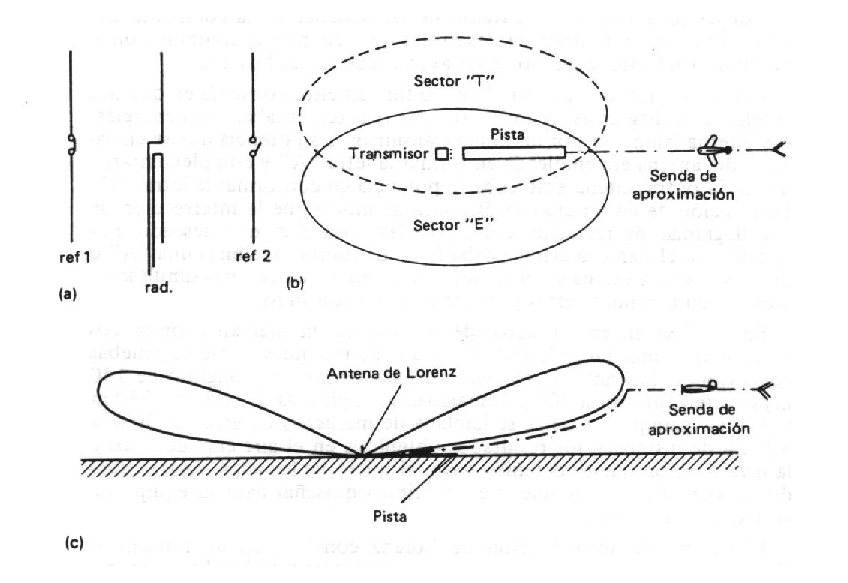
\includegraphics[width=0.8\textwidth]{06.radionavegacion/Imagenes/06.02.vor.imagenes/Loran.eps}
    \caption{El sistema de aproximaci\'on de Lorenz.
	(a) Dispositivo de antenas. (b) Modelo de radiaci\'on. \\(c) Diagrama polar vertical y senda de aproximaci\'on.
}
    \label{fig:sistema.lorenz}
\end{figure}

En 1917 se realizaron experiencias en Alemania con barcos y cinco a\~nos m\'as tarde, Keibitz las realiz\'o con aviones. Aunque en tierra se hablaba de un margen de error de 30 m a 3,5 km de distancia, los resultados obtenidos fueron dudosos y la investigaci\'on qued\'o detenida hasta comienzos de la d\'ecada de 1930 cuando la compa\~n\'ia us\'o de nuevo el principio equise\~nal para su equipo de aproximaci\'on de VHF.

Este equipo de aproximaci\'on de Lorenz consist\'ia en un transmisor de VHF situado en la cabecera de la pista de aterrizaje y trabajaba a una frecuencia de aproximadamente 33 Mhz. Este sistema alimentaba un dipolo vertical a cuyos lados, formando \'angulo recto con la pista, se situaba un elemento reflector. El punto medio de cada uno de estos elementos reflectores estaba interrumpido y puenteado por un conjunto de contactos de rel\'e que operaban en oposici\'on, esto es, si un conjunto de contactos se encontraba cerrado el otro estar\'ia abierto, manteniendo sin funcionar ese reflector.

\begin{minipage}[c]{0.5\linewidth}
Operando sobre los rel\'es, el diagrama de radiaci\'on pod\'ia ser trasladado de uno a otro lado. Ambos diagramas se interseccionaban sobre la l\'inea central de la pista  (Figura \ref{fig:sistema.lorenz}). La manipulaci\'on de los receptores se hac\'ia de modo que uno de ellos se manten\'ia en funcionamiento un per\'iodo de tiempo tres veces mayor que el otro; as\'i, cuando un piloto se aproximaba a la pista ligeramente fuera de rumbo, escuchaba una serie de ``\emph{E}'' ($\cdot \, \cdot \, \cdot$) o de ``\emph{T}'' ($- \, - \, -$) que se fund\'ian en un tono continuo ($- \cdot - \cdot - \cdot$) si se encontraba en el rumbo adecuado (Figura \ref{fig:seniales.lorenz}).

\end{minipage}
\begin{minipage}[c]{0.5\linewidth}
\centering
  \includegraphics[width=0.9\linewidth]{06.radionavegacion/Imagenes/06.02.vor.imagenes/Lorenz_beam.png}
  \captionof{figure}{ Se\~nales de Lorenz }
  \label{fig:seniales.lorenz}
\end{minipage}

 Este sistema se denomin\'o \emph{Ultrakurzwellen-Landefunkfeuer} (LFF), o radiobaliza de ondas ultra-cortas para aterrizaje.

El receptor del avi\'on estaba dotado de un medidor de intensidad de se\~nal y pod\'ia obtenerse una gu\'ia de la senda de planeo siguiendo un contorno de igual intensidad de campo.

Este sistema se puso en funcionamiento tambi\'en en Inglaterra con \'exito y se mantuvo en servicio hasta principios de 1960.

En Estados Unidos se investig\'o, por la misma \'epoca, un sistema de antenas ortogonales mediante se\~nales enclavadas. Este m\'etodo generaba cuatro rumbos independientes por cada estaci\'on y se le atribu\'ia una buena apreciaci\'on. 

Desde 1923 a 1926 se continu\'o esta l\'inea, descubri\'endose que utilizando un goni\'ometro transmisor junto con cuadros Bellini-Tosi, los rumbos pod\'ian ser desplazados casi a cualquier direcci\'on deseada. El \'exito del sistema fue tal que a comienzos de 1926 se emprendi\'o la labor de instalar un sistema de estas radiobalizas para trazar el creciente n\'umero de l\'ineas a\'ereas dentro de ese pa\'is. 

Posteriormente se encontr\'o que el sistema de antenas Bellini-Tosi presentaba errores de m\'as de 40 grados en condiciones nocturnas desfavorables, pero su sustituci\'on por antenas Adcock resolvi\'o este problema. En 1944 exist\'ian m\'as de 300 de estos equipos que permanecieron en servicio hasta ser reemplazados por el VOR.


Debido a los problemas inherentes al manejo de radiofaros omnidireccionales de frecuencias medias (efectos nocturnos, etc) en 1937 la U.S. Civil Aeronautics Administration llevó a cabo una serie de pruebas con el uso de VHF para radiofaros omnidireccionales. Las primer las pruebas usaban una frecuencia de 63 MHz y los resultados fueron prometedores, pero surgieron problemas debidos a efectos de reflexión bajo condiciones de propagaci\'on anormales y, en consecuencia, la frecuencia fue elevada a 12S MHz. Aunque todavía subsistían algunos problemas con los sistemas de cuatro rumbos, el trabaJo con VHF había demostrado que el equipo que trabajaba con estas frecuencias era capaz de obtener mejores resultados que el de MF. De todos modos, un problema importante que quedaba por resolver era la desorientación que experimentaba un piloto cuando perdía sus marcaciones cerca de un radiofaro de cuatro rumbos,  por eso se investigó la viabilidad de un sistema de radiofaro de dos rumbos, en el cual se emitian a la vez dos modelos de radiación que conformaban cuatro rumbos distintos. Típicamente podía consistir en un rumbo este-oeste definido por señales de 150 Hz y otro norte-sur de 90 Hz, separándose estas señales mediante filtros en el receptor del avión para alimentar diferencialmente un medidor con el cero en posición central. Esto se conoció como rumbo visual. Adicionalmente se instrumentaron un par de rumbos norte-sur en ángulo recto usando senales interconexionadas del tipo de Lorenz.% (D y U)

Hacia 1936 tambi\'en se consideró un radiofaro que radiaba un n\'umero infinito de rumbos, que era esencialmente un retorno al radiofaro giratorio.

Dicho radiofaro empleaba un sistema en el que el diagrama polar horinzontal tenía forma de cardioide, con la propiedad de que al girar, la intensidad de la señal en cualquier estación receptora variaba sinusoidalmente. El diagrama giraba a 60 Hz. La onda sinusoidal recibida era separada en dos partes en cuadratura de fase, que eran conectadas a las placas
de deflexión de un tubo de rayos catódicos. Esto producia una traza
circular, cada punto de la cual estaba asociado con el instante correspondiente a 
alguna orientaci\'on particular del diagrama espacial, pero sin
ningún punto de referencia. Este fue suministrado al principio introduciendo una discontinuidad en la se\~nal cuando el m\'aximo del diagrama
giratorio pasaba por el norte verdadero, siendo el resultado una deflexi\'on radial en la traza que,
 de otro modo, sería circular, proporcionando así una indicación del rumbo. 

En los primeros trabajos sobre dicho radiofaro se usaba una frecuencîa de 6,5 MHz, 
pero en vista de la tendencia en favor del uso de VHF
cesaron las pruebas con esta frecuencia y posteriormente se usaron frecuencias en la banda de 125 MHz.

Una versi\'on pasterior del equipo sustituía la discontinuidad instantánea de referencia
 por una modulaci\'on a 60 Hz de una subportadora de 10 kHz cuya fase se hacía coincidir con el diagrama
 giratorio en el norte verdadero.

En el receptor se comparaban las fases de la se\~na1 de referencia y de
la se\~nal g\'irada, correspondiendo la diferencia de fase con el rumbo
del receptor. Debido a esta modificaci\'on en la se\~nal de referencia 
se dej\'o de usar como \'indicador el tubo de rayos catódicos, 
que fue sustituido
por un medidor de fase con \'indicac\'i\'on azimutal.

Esto era, en esencia, el VOR que se usa hoy día, consist\'iendo las
principales variaciones posteriores en un cambio en la frecuencia para
usar la banda de 112,0 MHz a 117,9 MHz, en una reducción de la velocidad 
de rotaci\'on del d\'iagrama girator\'io y en una modulación de referenc\'ia
 de 30 Hz usando 9960 Hz para la frecuencia subportadora.

 \begin{myboxRojo}{Desarrollos durante la Segunda Guerra Mundial}

   {\footnotesize   

     \begin{minipage}[c]{0.65\linewidth}

     En el período de este conflicto se produjeron avances notables para el guiado y la navegaci\'on a ciegas de las aeronaves con el fin de realizar bombardeos de precisi\'on. 

Los alemanes utilizaron el principio del sistema de aproximación Lorenz para sus raids de bombardeo a ciegas, principalmente el 
Knickebein (``\emph{Pierna torcida}'') y el X-Ger\"{a}t (``\emph{Aparato-X}''),
durante la ofensiva de bombardeo sobre las ciudades de Inglaterra en el 
invierno de 1940/41.

El X-Ger\"{a}t era muy similar al LFF de Lorenz, siendo mucho m\'as direccional y con mayores alcances. Usando las mismas frecuencias permit\'ia a los aviones utilizar los emisores LFF ya instalados, pero se necesitaba un segundo emisor para ubicar una localizaci\'on.


\end{minipage}
\begin{minipage}[c]{0.35\linewidth}
  \centering
\includegraphics[width=0.9\linewidth]{06.radionavegacion/Imagenes/06.02.vor.imagenes/sottisville-x-geret.jpg}
\captionof{figure}{\footnotesize Modo de uso del X-Ger\"{a}t para posicionar Coventry}
\label{fig:Xgerat}
\end{minipage}


Estos sistemas utilizaban haces cruzados de radiondas de las mismas caracter\'isticas pero de diferentes frecuencias, lo que permit\'ia al piloto calcular su velocidad, desde el momento en que cruzaba la se\~nal y al cruzar la señal principal, luego le indicaba cuando liberar su cargamento.
Los c\'alculos se efectuaban mediante una computadora mec\'anica.

Posteriormente Lorenz modific\'o este sistema creando el sistema de guiado lateral 
Viktoria/Hawaii 
para el misil V-2.

}

\end{myboxRojo}


\subsection{Introducci\'on}
\label{sec:introduccion.vor}

VOR es un acr\'onimo para la frase "\textbf{\textit{VHF Omnidirectional Range}}", que en castellano significa Radiofaro Omnidireccional de VHF. Es un tipo de radioayuda a la navegaci\'on que utilizan las aeronaves para  para delinear aerovías en colaboración con el DME.

Desarrollado en Estados Unidos a partir del radiofaro giratorio de los años veinte, se reconoció como estándar internacional en 1949 y, por lo tanto, ha reemplazado al radiofaro internacional de MF.


\subsection{Principio de funcionamiento}
\label{Principio de funcionamiento}

El principio de funcionamiento del VOR es similar al de un faro de navegaci\'on mar\'itima.

\begin{minipage}[c]{0.6\textwidth}
El faro es una torre alta situada en las costas o en las cercanías de esta, donde se disponen las rutas de navegación de los barcos, que cuenta con un foco de luz muy potente en su parte superior cuya misión es la de guiar por las noches a los navegantes durante sus viajes, es decir, la prinicipal función de un faro es la de guía.

La mencionada lámpara cuenta con lentes de Fresnel que se caracterizan por su gran apertura y una corta distancia focal y cuyos anchos, color y separación variará de acuerdo al faro que se trate.

Mientras el faro está en funcionamiento en la oscuridad la mencionada lámpara emite haces de luz que giran a 360 grados. Entonces, desde la distancia en la cual se encuentren los barcos visualizarán no solamente la luz del faro sino también los colores y los intervalos de haces de luz que presenta la misma. Todo faro tiene su propia frecuencia de emisión de luz que lo hace único. De esta forma los marinos, consultando la correspondiente guía de faros, pueden determinar que faro están viendo y por lo tanto la zona donde navegan.
\end{minipage}
\begin{minipage}[c]{0.4\textwidth}

  \centering
  \includegraphics[width=0.9\linewidth]{06.radionavegacion/Imagenes/06.02.vor.imagenes/faro-alejandria.jpg}
  \captionof{figure}{El faro de Alejadr\'ia \\{\small (reconstrucci\'on)}}
  \label{fig:faro.alejandria}

\end{minipage}

En función de cómo se emite la señal luminosa, los faros se clasifican en: Faro de luz fija, faro de destellos, faro de luz centelleante, faro de grupos de destellos, faro de grupos de ocultaciones, faro de luz alternativa. Según la potencia de luz emitida y la altura en metros sobre el nivel del mar se obtiene el alcance geográfico, que no es más que la distancia máxima a la que se ve la luz que emite.

Los colores universalmente adoptados para emitir luz en los faros son el blanco, verde y rojo. Puede darse el caso, bajo ciertas condiciones atmosféricas, que la luz blanca o la verde adquieran un tono rosado.


El faro es un elemento célebre y útil desde la época de los Romanos, recordado es el faro de Alejandría e incluso esta civilización  supo construir en la entrada de los puertos torres sumamente altas que imitaban de alguna manera al mencionado Faro de Alejandr\'ia (Figura \ref{fig:faro.alejandria}). En el siglo XIX se produciría el gran salto de calidad de los faros con el invento del físico francés Agustin Fresnel. Actualmente los faros son operados a distancia y de manera automática.


El faro más antiguo que se encuentra en funcionamiento es el de la Torre de Hércules ubicado en la península de La Coruña, en Galicia; su alto es de 68 metros, data del siglo I y es el único faro romano en pie.

Volviendo al sistema VOR, la antena de la estaci\'on emite una se\~nal de radiofrecuencia VHF en todas direcciones, que es recibida por el equipo VOR de cualquier aeronave que se encuentre dentro del rango de alcance (max. unos 240 km) y tenga sintonizada la frecuencia de dicha estaci\'on (que puede variar de 108 a 118 MHz).

\begin{figure}[!b]
 \centering
 \subfigure[D-VOR/DME ground station. Identificaci\'on "PEK" (Beijing)]
   {
   \includegraphics[height=5.5cm]{06.radionavegacion/Imagenes/06.02.vor.imagenes/Vor_beijin.jpg}
   \label{fig:Vor_de_Beijin}
   }
 \subfigure[Esquema estaci\'on terrestre]
   {
   \includegraphics[height=5.5cm]{06.radionavegacion/Imagenes/06.02.vor.imagenes/VORGroundStation.jpg}
   \label{fig:Vor.estacion.terrestre}
   }
 \caption{Estaciones VOR }
\end{figure}


La estaci\'on de tierra posee un diagrama de radiaci\'on din\'amico, transmite dos se\~nales VHF en el rango anteriormente mencionado. La radiofrecuencia emitida por un VOR lleva tres se\~nales codificadas. Una es la identificaci\'on de la estaci\'on en c\'odigo Morse \footnote{El c\'odigo Morse es un sistema de representaci\'on de letras y n\'umeros mediante se\~nales emitidas de forma intermitente.}, que permite al piloto saber de cu\'al estaci\'on se trata. Las otras dos son ondas senoidales de 30 Hz cuyas fases var\'ian entre si. Se les llama se\~nal de referencia y se\~nal variable respectivamente. La referencia mantiene siempre su fase constante, mientras que la variable cambia su fase seg\'un la direcci\'on en la que sea emitida. Dicha direcci\'on se mide como un azimut, es decir, se divide en 360 grados alrededor de la antena VOR contando en sentido horario a partir del norte magn\'etico terrestre, punto en el cual la se\~nal de referencia y la variable tienen fase id\'entica. De esta manera se puede visualizar una antena VOR como el punto desde el cual parten 360 l\'ineas de direcci\'on, a las que se les llama radiales.

El equipo VOR en la aeronave recibe la se\~nal VOR y decodifica sus tres se\~nales. Compara la se\~nal de referencia con la variable y determina la diferencia de fase entre las dos. De esta manera puede conocerse en qu\'e radial del VOR sintonizado se encuentra la aeronave con respecto al norte magn\'etico terrestre.

El VOR se utiliza en la aeron\'autica para navegar seg\'un el vuelo IFR \footnote{Recibe el nombre de Reglas de Vuelo Instrumental (m\'as conocido por sus siglas en ingl\'es, IFR), el conjunto de normas y procedimientos recogidos en el Reglamento de Circulaci\'on A\'erea, que regulan el pilotaje de aeronaves en condiciones de visibilidad reducida. Se trata del m\'etodo de navegaci\'on alternativo a las Reglas de Vuelo Visual o VFR.}, siempre permaneciendo en radio con un CTA. Los VOR suelen ir acompa\~nados de DME (Distance Measurement Equipment, Equipo de Medici\'on de Distancia), \'estos son completamente independientes del sistema VOR y ayudan al piloto a saber la distancia que hay entre la aeronave y la estaci\'on VOR. El VOR \'unicamente se utiliza en la llamada "radio navegaci\'on" por lo que siempre hay unos procedimientos que seguir que los marca la carta aeron\'autica para dirijirse a un VOR. Por ejemplo en las SID o salidas normalizadas de un aeropuerto, en la respectiva carta se verifica el procedimiento de apoyo en la salida con los NDB y VOR para poderla realizar correctamente. El piloto debe saber volar bajo reglas de vuelo IFR a un VOR y desde un VOR, o cualquier radioayuda que sea: (NDB, VOR, ILS u otras como el TACAN \footnote{Las siglas TACAN significan  TACtical Air Navigation,  es un tipo de ayuda a la navegaci\'on de uso militar.}) \cite{VOR-Wikipedia}.

Desarrollado de un sistema anterior, Visual-Aural Range (VAR), el VOR se dise\~n\'o para proveer 360 rumbos desde y hacia la estaci\'on seleccionada por el piloto. Los antiguos transmisores de tubo de vac\'io con antenas rotadas mec\'anicamente se instalaron por todos lados en la d\'ecada de 1950 y en la de 1960 comenzaron a ser reemplazados por unidades de estado s\'olido. En este mismo per\'iodo se transformaron en el mayor sistema de navegaci\'on cuando reemplazaron a las viejas radiobalizas. Algunas de estas sobrevivieron como balizas no direccionales de baja o media frecuencia (NDB \footnote{Una Baliza No Direccional,  Non-Directional Beacon (NDB), es una estaci\'on de radio ubicada en un lugar conocido, utilizada como una ayuda para la navegaci\'on a\'erea o naval. Como su nombre implica, la se\~nal no provee informaci\'on direccional en contraste con nuevos tipos de ayudas como VOR. La se\~nal de una NDB copia el contorno de la curvatura de la tierra por lo que puede ser recibida a distancias mayores en latitudes menores, lo que constituye una ventaja sobre el sistema VOR. Sin embargo, la se\~nal NDB es afectada por condiciones atmosf\'ericas, terreno monta\~nosos, refracci\'on costera y tormentas el\'ectricas, particularmente a grandes distancias. A\'un con la aparici\'on de los sistemas VOR y GPS (Global Positioning System), las NDBs contin\'uan siendo las ayudas de navegaci\'on m\'as ampliamente usadas en el mundo. Las NDBs operan en el rango de frecuencias de 190 kHz a 535kHz (aunque tienen frecuencias reservadas en el rango de 190 a 1750 kHz) y una portadora modulada entre  400 o 1020 Hz. Entre la informaci\'on transmitida por una NDB se tiene:

\begin{itemize}
 \item Identificaci\'on por c\'odigo Morse entre 400 a 1020 Hz.
\item Informaci\'on de la Terminal A\'erea (Airfield Terminal Information Service = ATIS)
\item Servicio de informaci\'on clim\'atica de la Terminal A\'erea (Airfield Weather Information Service = AWIS), o, en una emergencia un controlador de tr\'afico a\'ereo activando la funci\'on de Presionar-para-hablar (Press-To-Talk = PTT), puede modular la portadora con la voz. El piloto utiliza su receptor ADF para escuchar las instrucciones desde la torre.
\end{itemize}
}).

En los aviones de hoy en d\'ia esto se realiza mediante la FMC, o MCDU seg\'un el fabicante del avi\'on, ya que intoducen directamente la SID y la FMC la realiza automaticamente sola. As\'i podemos llevar a cabo un vuelo, tanto de larga como de corta distancia entre dos puntos del mundo.

En las rutas a\'ereas comerciales m\'as transitadas, al igual que en las carreteras terrestres, hay cruces y curvas. Bajo estos ``\emph{cruces}'' y ``\emph{curvas}'' se suelen instalar estas estaciones VOR. Las ``\emph{carreteras a\'ereas}'' son los radiales de XXX grados que parten de un VOR y que normalmente llegan a otro VOR o incluso a una pista de aterrizaje.

El piloto puede ordenar al piloto autom\'atico: "\textit{Sigua el radial de 115 grados del VOR que transmite en la frecuencia 109.75 Mhz}.", y el avi\'on autom\'aticamente, cuando se cruce con el radial 115, lo seguir\'a hasta sobrevolar el VOR.

\begin{figure} [!hbt]
 \centering
 \includegraphics[width=0.750\textwidth]{06.radionavegacion/Imagenes/06.02.vor.imagenes/mapa_vor.jpg}
 % Mapa_VOR.eps: 0x0 pixel, 300dpi, 0.00x0.00 cm, bb=0 0 500 301
 \caption{Mapa con ruta y posici\'on de estaciones VOR}
 \label{Mapa_estaciones_VOR}
\end{figure}

En el mapa de la Figura  \ref{Mapa_estaciones_VOR} se puede ver una serie de radiobalizas VOR (los c\'irculos grandes) interconectadas entre si por rutas a\'ereas. Cada ruta a\'erea tiene marcado su nombre, altitud y rumbo (que coincide con el radial del VOR del que parte).


\subsection{Equipo de tierra}

\subsubsection{Principios de funcionamiento }

El transmisor es de tipo AM de diseño estándar excepto en el hecho de que el modulador debe ser capaz de trabajar a  frecuencias por encima de los 10 kHz. Para las ayudas en ruta, la potencia de salida es de 200 W, para servicio en aeródromos sólo se necesita 50 W.

La operación de un equipo VOR de tierra está basada en Ia diferencia de fase entre dos señales que emite: una de referencia y otra variable. Cada grado de variación de fase entre las señales, representa un grado de variación de posición del avión.

Los radiales de un VOR son infinitos, pero el equipo de a bordo solo es capaz de diferenciar 360 de ellos.

En una estación VOR, un sistema de monitores y dos transmisores, aseguran un servicio continuo de funcionamiento. Si la señal del equipo se interrumpe por cualquier causa, o varían sus fases, el sistema de monitores desconecta el equipo defectuoso, conectando a su vez un transmisor auxiliar y excitando una alarma en el panel de control que indica un fallo en el sistema. En la Figura \ref{fig:estaciones_VOR}  pueden verse estaciones de tierra. 

\begin{figure}[!htb]
  \centering
  \subfigure[Estación VOR]{
\includegraphics[keepaspectratio,height=4.5cm]{06.radionavegacion/Imagenes/06.02.vor.imagenes/Emisor_VOR.eps}}
  \subfigure[Estación VOR Beijin]{\includegraphics[keepaspectratio,height=4.5cm]{06.radionavegacion/Imagenes/06.02.vor.imagenes/Vor_beijin.jpg}}
  \caption{Estaciones VOR}\label{fig:estaciones_VOR}
\end{figure}


El equipo transmisor trabaja en VHF en la banda de 112 Mhz a 118 Mhz, en frecuencias que terminan en décimas pares o impares, y centésimas impares. Se podrán usar frecuencias comprendidas entre 108 Mhz y 112 Mhz cuando:

\begin{itemize}
\item Se usen en VOR de cobertura limitada únicamente

\item Se usen solo frecuencias que terminen bien en décimas pares o centésimas impares de Mhz

\item No se utilicen estas frecuencias para el sistema ILS.

\item No se ocasionen interferencias al ILS
\end{itemize}


\subsubsection{Cono de silencio}

En la emisión de las estaciones VOR se producen ciertas zonas ciegas donde la señal es nula. A estas zonas se las Ilama conos de silencio, y se encuentran localizadas sobre la estación. Cuando la aeronave la esté sobrevolando, no recibirá ningún tipo de señal. La amplitud de la zona de silencio, debido a su forma de cono invertido, se incrementa con la altura. De esta manera, un avión volando a 20.000' sobre una instalación VOR, permanecerá más tiempo en el cono de silencio que otro avión que lo esté haciendo a 10.000'.

\subsubsection{Clasificación y tipos de estaciones VOR}
\label{sec:clasificacion.y.tipo.estaciones.vor}

La clasificación de las estaciones VOR se efectúa de acuerdo con la altitud y distancia libre de interferencias a la que éstas pueden recibirse. Existen dos criterios sobre el particular: el de la FAA y el de OACI.

La clasificación americana de la F.A.A. es la siguiente:

\begin{itemize}
\item \textbf{T-VOR. VOR terminal o de recalada:} Las condiciones operativas de este primer tipo de VOR son tales que no debe ser usado para la navegación si la aeronave que desea sintonizarlo, está a más de 25 NM de Ia estación y a una altitud superior a 12.000'. A partir de esta distancia y altitud, sus indicaciones no son de fiar.
Los VOR de recalada se usan principalmente como ayuda a la aproximación a los aeropuertos, y nunca como ayudas de ruta.


\item \textbf{L-VOR. VOR de baja altitud:}  Este tipo de estación puede usarse con seguridad hasta una distancia de 40 millas náuticas y una altitud de 18.000 pies. Puede usarse, además de come ayuda a la aproximación como apoyo en ruta.


\item \textbf{H-VOR. VOR de gran altitud:} El H-VOR tiene un alcance de unas 40 millas náuticas por debajo de 18.000 pies y de 130 millas náuticas por encima de esta altitud, con un máximo de 156 millas náuticas a  75000 pies. Los alcances de los distintos tipos de VOR no deben confundirse con una mayor o menor potencia de emisión de las estaciones de tierra, pues ésta es prácticamente la misma para todos, situándose alrededor de los 200 W. 

\end{itemize}

Según OACI, únicamente hay dos tipos de instalación VOR. 

\begin{itemize}
\item \textbf{VOR-A:} Una aeronave recibirá las señales de este tipo de VOR, hasta una distancia de 100 millas náuticas por lo menos, y hasta un ángulo de elevación de 40 grados, siempre que no existan obstáculos entre la estación y dicha aeronave.

\item \textbf{VOR-B:} Esta estación VOR será recibida a una distancia de 25 millas náuticas y con un ángulo de 40 grados por lo menos.

\end{itemize}

\subsubsection{Volumenes de Servicio}
\label{sec:volumenes.de.servicio}

Una estaci\'on de VOR sirve a un volumen del espacio a\'ereo denominado \emph{Volumen de Servicio (Service volume)}. Algunos VOR poseen una peque\~na \'area geogr\'afica protegida de la interferencia de otras estaciones con la misma frecuencia (T-VOR), otros tienen protecci\'on hasta 130 millas n\'auticas (240,76 km) o m\'as. 

Las dimensiones de los volumenes de servicio de los distintos tipos de VOR  no deben confundirse con una mayor o menor potencia de emisi\'on de las estaciones de tierra, pues \'esta es pr\'acticamente la misma para todos, situ\'andose alrededor  de los 200 W, y se especifica para que el volumen especificado se provea una adecuada intensidad de se\~nal.

En los Estados Unidos se especifican tres volumenes de servicio normalizados (Standard Service Volumes - SSV): Terminal, Low, y High, es decir, seg\'un la clasificaci\'on de la FAA (Figura \ref{fig:volumenes.de.servicio}).


% \begin{table}[!h]\centering

% \caption{US Standard Service Volumes (extra\'ido de FAA AIM) }
% \begin{tabular}[!h]{|l|m{0.7\textwidth}|}  \hline
% {\bf SSV Class Designator} &	\textbf{Dimensiones} \\ \hline
% T (Terminal) &	%From 1,000 feet above ground level (AGL) up to and including 12,000 feet AGL at radial distances out to 25 NM.
% Desde 1000 pies desde el nivel de tierra (Above Ground Level - AGL) hasta los 12000 pies AGL con un radio de 25 millas n\'auticas \\ \hline
% L (Low Altitude) 	&%From 1,000 feet AGL up to and including 18,000 feet AGL at radial distances out to 40 NM .
% Desde 1000 pies AGL hasta 18000 pies AGL con un radio de 40 millas n\'auticas\\ \hline
% H (High Altitude) 	&From 1,000 feet AGL up to and including 14,500 feet AGL at radial distances out to 40 NM. From 14,500 AGL up to and including 60,000 feet at radial distances out to 100 NM. From 18,000 feet AGL up to and including 45,000 feet AGL at radial distances out to 130 NM. \\ \hline
% \end{tabular}
% \end{table}

\begin{figure}[!htb]
  \centering
  \includegraphics[width=0.7\textwidth]{06.radionavegacion/Imagenes/06.02.vor.imagenes/vor-service-volume-02.png}
  \caption{VOR. Volumenes de servicio}
  
  \label{fig:volumenes.de.servicio}
\end{figure}

Actualmente, existe gran cantidad de instalaciones VOR, por lo que en determinados lugares, a lo largo de una ruta, podría darse el caso de que dos estaciones, emitiendo en Ia misma frecuencia o en frecuencias muy cercanas, se interfirieran. 

En vistas a que esto no suceda, Ias áreas en las que estas interferencias son posibles, vienen indicadas en las cartas de navegación con eI símbolo MAA seguido de unas cifras que indican una altitud. La MAA o Altitud máxima autorizada, asegura la nítida recepción de una señal VOR  sin interferencias, y por supuesto, guardando la mínima separación de seguridad con el terreno.

La recepción de una señal interferida se hará evidente por falsas indicaciones en el receptor VOR, por oscilaciones de los indicadores y por silbidos agudos.

La única corrección posible a este inconveniente, es la sintonización e otra estación VOR que convenga a la ruta que se está volando. Realmente es muy difícil que dos equipos VOR cercanos transmitan en la misma frecuencia, pero en zonas de gran densidad de instalaciones, puede Llegar a suceder.

\subsubsection{Identificación de las estaciones VOR}

La señal de identificación de las estaciones VOR consiste en un tono de 1020 Hz que modula en amplitud a la portadora por medio de una señal de radiofrecuencia, la cual emite el indicativo de la estación en código Morse1. La identificación consiste en dos o tres letras transmitidas a una velocidad de 7 palabras por minuto, siendo emitidas una vez cada treinta segundos.

Los VOR que se identifican con dos letras en Morse, suelen ser los T-VOR, siendo los VOR de ruta los que lo hacen con tres letras.

En estaciones más modernas, se puede proporcionar un canal de comunicaciones unilateral tierra-aire, simultáneo al de navegación. Ambos canales se emiten a través de la misma portadora de radiofrecuencia. La emisión de las estaciones es del tipo A9 o modulación de frecuencia. Este nuevo canal de radiotelefonía se utiliza para la identificación del equipo en forma oral. Otros usos que se le pueden dar son la emisión de informes de meteorología, pista en servicio, viento, QNH, estado operacional del aeropuerto. Este servicio se conoce bajo la denominación ATIS (Automática Terminal Information Service).

Cuando un VOR se identifica en radiotelefonía y radiotelegrafía simultáneamente, lo hará tres veces cada treinta segundos, dos en Morse y una oralmente.

Hay que señalar que cuando se sintonice una estación VOR, es muy importante llevar a cabo su identificación y comprobaría regularmente. Cuando la estación no da indicativo, o este no es audible, hay que desconfiar de las indicaciones que se presentan en el equipo de a bordo. Por otra parte, será necesario saber que cuando se está procediendo a la reparación o mantenimiento de los equipos de tierra, el emisor no transmite identificación.



\subsection{Equipo de a bordo}

Cuatro son los componentes del equipo de a bordo del sistema VOR. Estos son:

\begin{multicols}{2}
  
\begin{itemize}
\item Antena 

\item Receptor


\item Servoamplificador 

\item Indicador

\end{itemize}
\end{multicols}

\subsubsection{Antena }

La antena del equipo VOR no tiene complicación alguna y tan solo cabe destacar su forma en V y que, casi siempre, va instalada en el estabilizador vertical de cola o en la parte superior del fuselaje. Su misión consiste en recibir las líneas de flujo electromagnético emitidas por la estación de tierra y transmitirlas al receptor.

\subsubsection{Receptor }

La función del receptor consiste en interpretar o medir, con ayuda de los indicadores, la diferencia de fase entre las dos señales la de referencia y la  variable, emitidas por el equipo de tierra. Los modernos receptores suelen tener los siguientes mandos de control:

\subsubsection{On/off-volumen}
Cuando este interruptor está en su posición OFF, el receptor no recibe energía, y  por tanto, permanece inactivo. Cuando su posición es ON, está ya preparado para su funcionamiento. Si se sigue girando este interruptor cuando está en ON, el  resultado es un aumento de volumen en la recepción de la estación selectada. Este mando de volumen no afecta, aunque esté en su posición de mínimo, a la señal de navegación que Ilega al indicador.

\subsubsection{Selector de frecuencias}
Consiste en dos ruedas con las que se selectan las frecuencias. Una de ellas selecciona las comprendidas entre 108 y 136 Mhz, y la otra selecciona Khz o centésimas de Mhz. Este selector permitirá, pues, selectan un canal entre 560 posibles.

Aunque el emisor del equipo VOR trabaja casi siempre entre 112 y 118 Mhz, el receptor de a borde cubre la banda comprendida entre 108 y 136 Mhz, con lo que es capaz de admitir frecuencias para operar en las funciones ILS, VOR y comunicaciones en radiotelefonía aire - tierra y tierra-aire. La banda de frecuencias que se puede sintonizar en el receptor tiene la siguiente distribución:

\begin{itemize}
\item De 108 Mhz a 112 Mhz, para ILS y VOR 

\item De 112 Mhz a 117,9 Mhz, para VOR.

\item De 118 Mhz a 135,9 Mhz, para radiotelefonía

\end{itemize}

El motivo de que el receptor sea capaz de cubrir las tres funciones mencionadas, radica en la necesidad de condensar al máximo el equipo de cabina. De esta manera se evita el tener que instalar un receptor independiente para cada equipo.

\subsubsection{Ventanilla selectora}
En ella se lee la frecuencia selectada.

\subsubsection{Interruptor filtro de identificación (Ident)}
El tono de identificación de la estación de tierra es filtrado, mediante la presión del interruptor IDENT, cuando es muy necesaria una recepción nítida y clara de dicho tono.

\begin{figure}[!hb]
  \centering
  \subfigure[Antena recepción señales VOR]{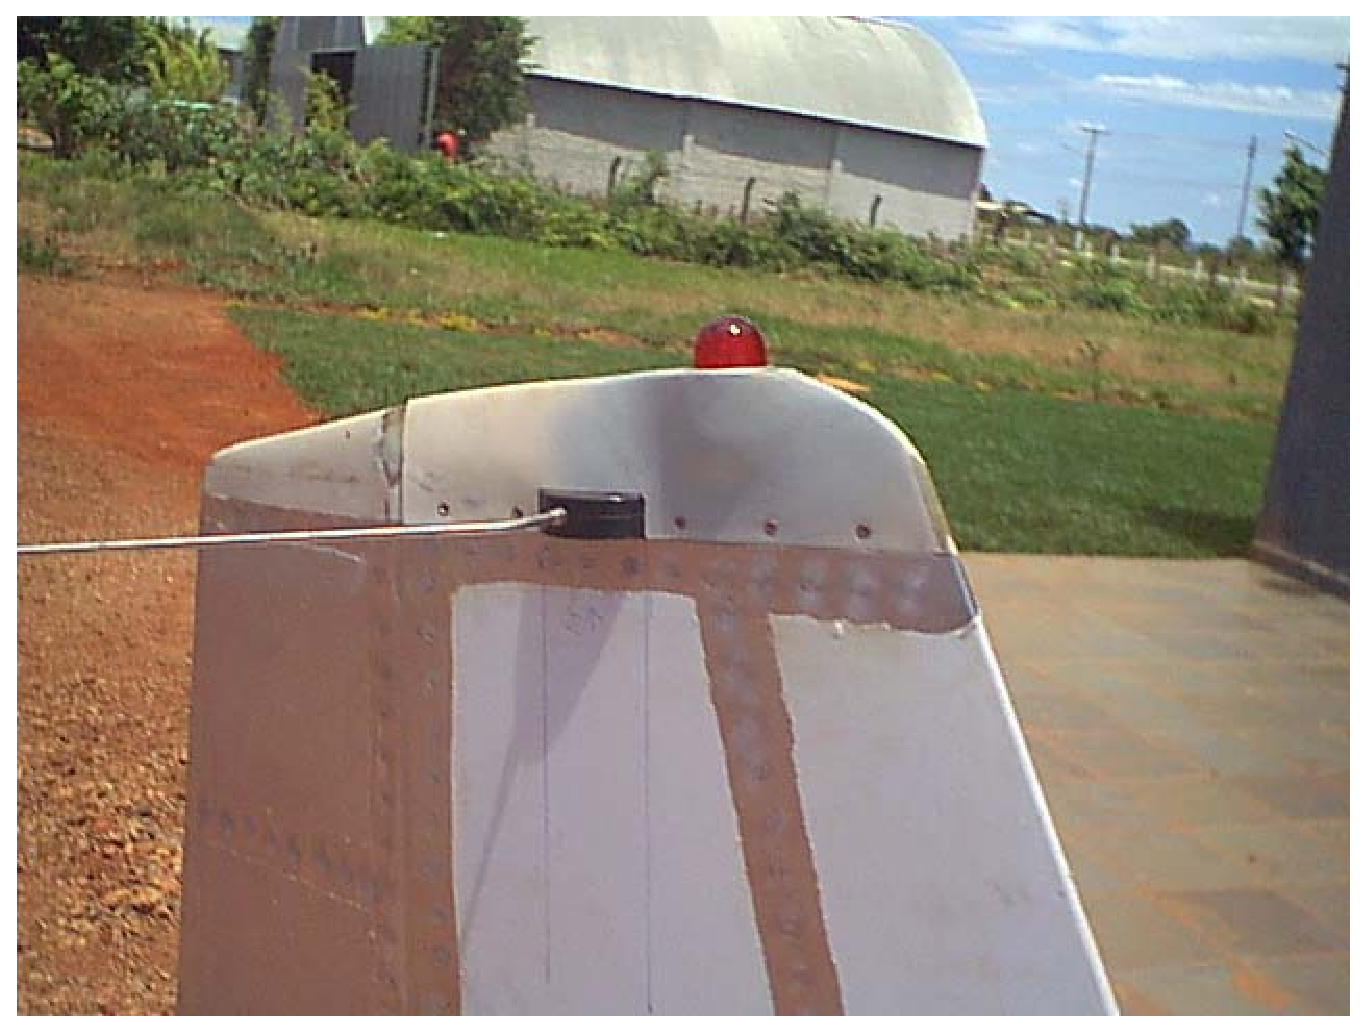
\includegraphics[width=0.3\textwidth]{06.radionavegacion/Imagenes/06.02.vor.imagenes/Antena_Vor_empenaje_vertical.eps}}
  \subfigure[Receptor (Nav-Com)]{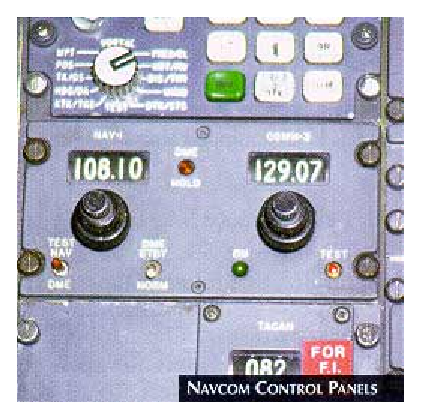
\includegraphics[width=0.3\textwidth]{06.radionavegacion/Imagenes/06.02.vor.imagenes/Nav-com.eps}}
  \subfigure[Indicador VOR (¡modelo obsoleto!)]{
\includegraphics[width=0.3\textwidth]{06.radionavegacion/Imagenes/06.02.vor.imagenes/Indicador-vor-viejo.eps}}
  \caption{Equipo a bordo sistema VOR}
\end{figure}


\subsection{Servoamplificador}
La energía electromagnética llega desde el emisor de tierra hasta la antena de a bordo. Desde allí es enviada al receptor, donde es convertida en impulsos eléctricos. Estos impulsos no bastarán para producir las deflexiones necesarias en indicador VOR, por lo que tienen que ser tratados por un servoamplificador. Una vez amplificados los impulsos ya pueden ser transmitidos al indicador.

\subsection{Indicador VOR}

La función única del indicador VOR, es mostrar al piloto su situación con respecto a la estación de tierra en cualquier momento. La información es clara y precisa y da, constantemente, indicaciones de mando, o da qué debe hacer el piloto para mantener a la aeronave sobre una ruta determinada. 

\begin{figure}[!htb]
  \centering
  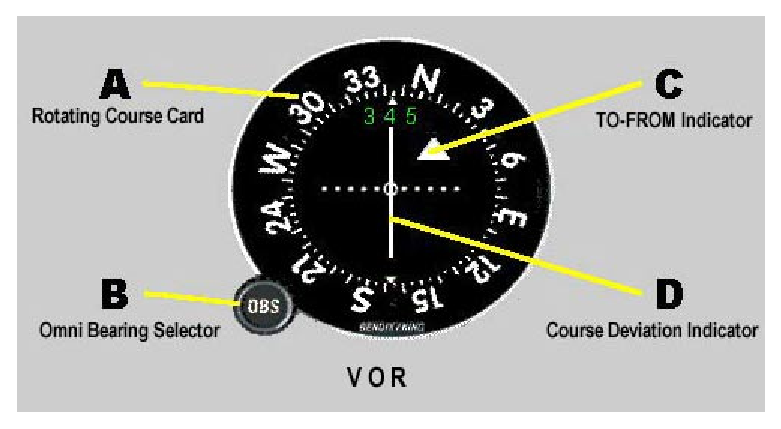
\includegraphics[width=\textwidth]{06.radionavegacion/Imagenes/06.02.vor.imagenes/vor_indicator.eps}
  \caption{Partes de un indicador VOR}
  \label{fig:indicador-vor}
\end{figure}

Aunque hay muchos tipos de indicadores VOR, este estudio se ce\~nir\'a a la descripci\'on de un equipo moderno que consta de los siguientes elementos:

\begin{itemize}

\item \textbf{Selector de rutas (OBS):} Con el OBS (Omni - Bearing Selector), el piloto puede seleccionar la ruta que desee con el fin de interceptarla y acercarse o alejarse por ella, de una estación VOR. El OBS es un pequeño mando adosado a la caja del instrumento, y con él se gobierna la rotación de la carta o rosa graduada en 360 grados que va instalada en el interior del indicador VOR.


\item \textbf{Bandera TO-0FF-FROM:} La misión de la bandera TO - OFF - FROM, es resolver los 180 grados de ambigüedad que tendría la ruta seleccionada, mostrando si ésta, una vez haya sido interceptada, conducirá al avión hacia (TO) la estación, o por el contrario, si le alejará de ella (FROM). Si la aeronave está fuera del alcance de la estación de tierra, y por tanto no recibe una señal fiable, el indicador  TO - FROM desaparecerá, siendo sustituido por la palabra OFF. Este indicador será también visible cuando la aeronave se encuentre en el cono de silencio de la estación VOR, o cuando la ruta seleccionada se encuentre entre 85 grados ó 90 grados de distancia de la posición real del avión. La banderilla TO - OFF - FROM es activada por medio de energía eléctrica procedente de las fuentes principales del avión (corriente continua).


\item \textbf{Indicador de desvío de ruta (CDI):} Una vez una ruta haya sido selectada e interceptada, el CDI (Course Desviatìon Indicator), indicará al piloto si la está siguiendo correctamente, o si por el contrario se ha desviado de ella. Si el avión está sobre la ruta seleccionada, al CDI estará centrado en el instrumento. El piloto puede pensar en el CDI como en un pedacito de ruta trasladado a su indicador de a bordo. Considerándolo de esta manera, cuando el avión se encuentre a la derecha de la ruta seleccionada, el CDI estará desplazado a la izquierda del instrumento. En el caso opuesto, cuando e1 avión esté volando a la izquierda de la ruta, el CDI estará desplazado a la derecha del instrumento. En cualquier caso, el CDI indicará a qué lado del avión está la ruta que el piloto haya seleccionado y hacia dónde tiene éste que virar para reinterceptarla. En el centro del instrumento y en cada una de sus mitades, hay dibujados cinco puntos que indican la distancia en grados entre la ruta seleccionada y el avión. Un desplazamiento del CDI de dos puntos, indicará una separación de cuatro grados. Cada punto equivale, pues, a dos grados. Es evidente que el haz que cubre el instrumento en cada lado de la ruta seleccionada, es de diez grados.

\item \textbf{Pulsador de TEST:} Sirve única y exclusivamente para medir la seguridad de las indicaciones del CDI. Haciendo uso del pulsador, el CDI sufrirá un desplazamiento determinado hacia uno de los lados del instrumento, lo cual indicará su buen funcionamiento. En caso de que el CDI no reaccionara de esta manera, eI instrumento no sería de fiar. En muchos instrumentos eI TEST va instalado en el mismo mando que el OBS.

\item \textbf{Fiel:} El fiel es un punto grabado en la parte superior de la caja del instrumento, bajo el cual, el piloto situará la ruta deseada.

\item \textbf{Fiel de ruta reciproca:} Este fiel es diametralmente opuesto al anterior, y sirve al piloto como recordatorio de la ruta recíproca a la que lleva selectada.

\item \textbf{Referencias de 90 grados:} Son otros dos puntos situados a derecha e izquierda del indicador, dando referencia de cuáles son las rutas situadas a 90 grados de la ruta seleccionada.


\end{itemize}



\subsection{Interpretación de las presentaciones VOR}

Tres componentes del indicador VOR, trabajando conjuntamente, dan al piloto una línea de situación con respecto a la estación de tierra o a cualquier ruta seleccionada en el equipo de a bordo. Estos tres elementos son el selector de rutas OBS, e1 CDI y el indicador o bandera TO-FROM. Al contrario que una aguja de ADF que apunta continuamente a la estación, estos tres componentes no se ven afectados por el rumbo del avión para una posición dada. En consecuencia, el avión y, por tanto, el girodíreccíonal, deben ser orientados según la presentación VOR para obtener una indicación correcta de la dirección de la ruta. Por ello, el piloto deberá efectuar una serie de procedimientos que le permitan acercarse o alejarse de una estación sin posibles errores.

\begin{figure}[htb]
  \centering
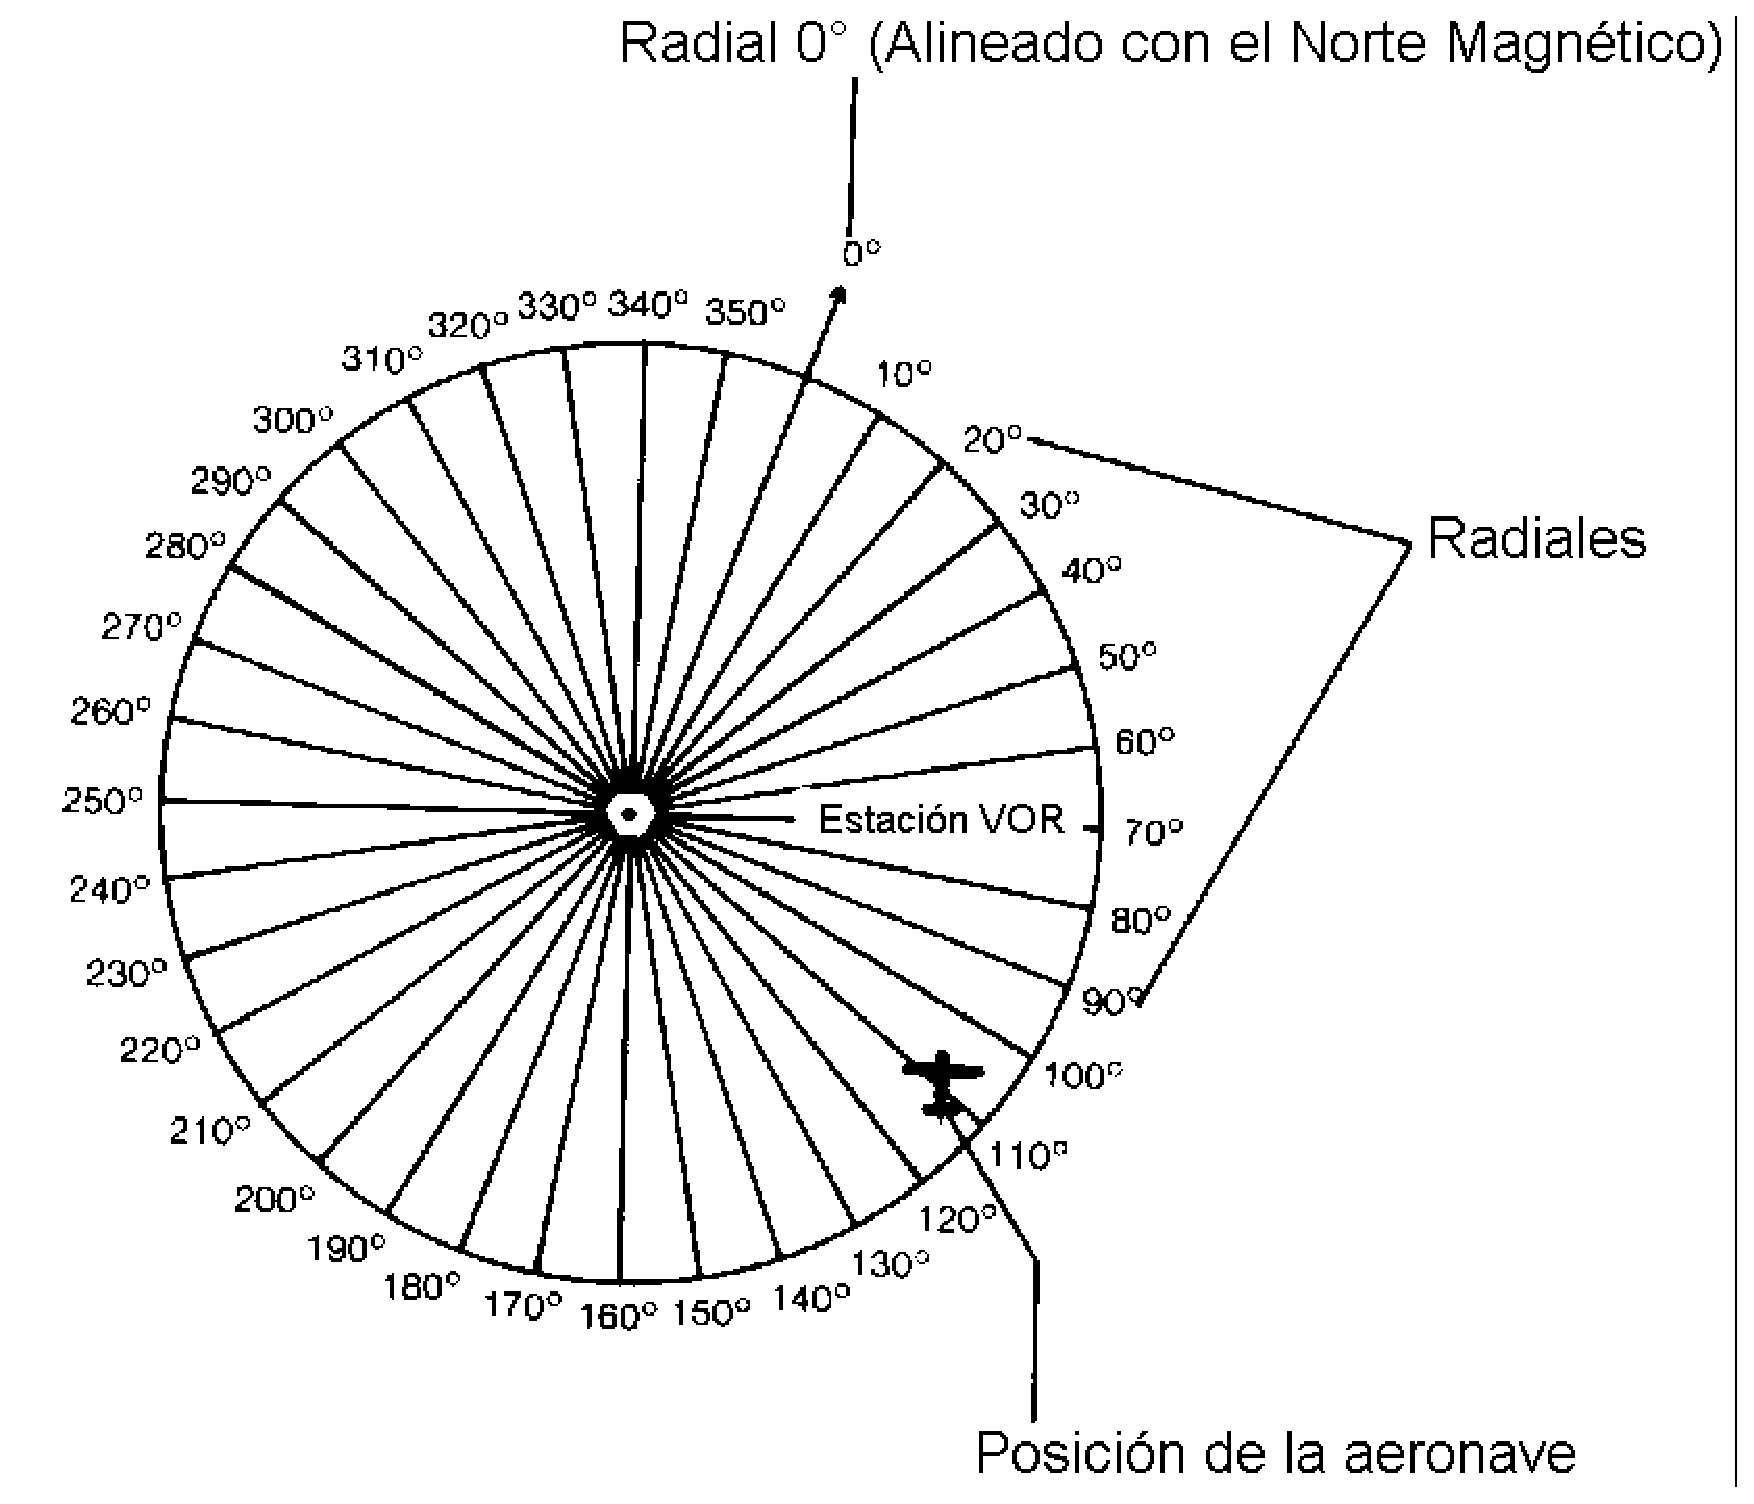
\includegraphics[keepaspectratio,width=0.8\textwidth]{06.radionavegacion/Imagenes/06.02.vor.imagenes/radiales-vor.eps}
  \caption{Radiales de una estación VOR}
  \label{fig:radiales-vor}
\end{figure}


Si el piloto, desde un punto cualquiera, desea dirigirse a una estación VOR, selectará su frecuencia y la identificará. Con el OBS girará la rosa del indicador VOR de a bordo hasta que el CDI quede centrado y aparezca en la ventanilla la bandera con la palabra TO. Cuando esto suceda, mírará debajo del fiel para conocer cuál es su ruta magnética de acercamiento (TO) a la estación. Hará virar su avión hasta que su rumbo magnético coincida con la ruta magnética que señala el fiel del VOR. En el viraje, el CDI, probablemente y dependiendo de la distancia a la estación, habrá sufrido un pequeño desplazamiento, por lo que e1 piloto volverá a centrarlo de nuevo siempre en TO, y tomará el nuevo rumbo magnético que coincida con la Ruta magnética que señale ahora el fiel de indicador VOR. Manteniendo el CDI centrado en esta posición, indudablemente, el avión procederá en arribada a la estación. 

La marcación magnética o QDR del avión con respecto a 1a estación, será la recíproca a la ruta magnética que lleve el avión en ese momento. Si la aeronave prosigue acercándose a la estación, llegará un punto en el que penetre en su cono de silencio. El tiempo que permanezca en él dependerá, lógicamente, de la velocidad y altitud a las que vuele el avión. En ese punto, el CDI oscilará debido a que el instrumento no recibe ningún tipo de señal desde tierra, apareciendo casi simultáneamente la banderilla OFF en ventanilla. Al atravesar el cono de silencio, y suponiendo que el avión haya mantenido constante su rumbo magnético, la bandera OFF se ocultará, apareciendo en su lugar la palabra FROM, y el CDI volverá a centrarse. A partir de esta punta, el piloto sabrá positivamente que ha sobrevolado la estación y que ya se está alejando de ella por la ruta magnética que señala el fiel del indicador VOR.

Evidentemente toda la maniobra se ha descrito suponiendo que el viento es inexistente. En caso de que éste tuviera fuertes componentes,

A pesar de que el piloto pudiera mantener el CDI centrado en el instrumento, el rumbo magnético del avión y la ruta magnética, por supuesto que no coincidirían.

Como explicación complementaria, puede decirse que para una posición dada del avión, una rotación de 360 grados  de la rosa del indicador VOR, efectuará un ciclo completo de cambios en las indicaciones dei CDI y de la bandera TO-OFF-FROM. Este ciclo sería el mismo que el que podría observarse si fuera el avión el que se desplazara en círculo alrededor de la estación con una ruta magnética fija seleccionada bajo el fiel del instrumento.

Al llevar a cabo esta maniobra, el CDI se centrará en dos puntos distintos que serán opuestos -separados 180 grados  - los cuales constituyen la línea de situación del avión con respecto a la estación. En uno de los puntos aparecerá la banderilla TO. Si ahí el piloto virara su avión hacia la ruta magnética señalada bajo el fiel del VOR, procedería en arribada a la estación.

El otro punto en el que el CDI se centre estará a 180 grados del primero y  será visible la bandera con la palabra FROM. Si en ese punto el avión virara hacia la ruta magnética señalada en el fiel del VOR, procedería en alejamiento de la estación. 

El piloto deberá tener especial cuidado al trabajar con el equipo VOR. Podría darse el caso de estar alejándose de la estación llevando en ventanilla la palabra TO, o viceversa, acercándose en ella en FROM

Esto sería causado por una selección errónea de la ruta magnética deseada. 

Hay que tener siempre presente que en una aeronave que se está alejando de una estación VOR, la ruta magnética seleccionada y el Radial VOR, coinciden. Si por el contrario se está acercando a la estación, la ruta magnética seleccionada es el Radial VOR opuesto al que está realmente sobrevolando la aeronave.



\subsection{HSI (Horizontal Situation Indicator) Indicador de situación horizontal}

Uno de los instrumentos que pueden realizar la función de indicadores VOR es el HSI.

\'Este es uno de los componentes del Director de Vuelo (FLIGHT DIRECTOR) y actúa como instrumento indicador para las señales de radionavegación que llegan a bordo de la aeronave. Este instrumento puede también ser instalado independientemente del sistema Director de Vuelo y es susceptible de ser usado como indicador de las estaciones VOR, ILS y ADF.

Por otra parte, el HSI presenta las indicaciones de sistemas como el CLC 3D, el INS, el OMEGA y el DOPPLER, sirviendo las órdenes de las computadoras de navegación de estos equipos.


\begin{figure}[!h]
  \centering
  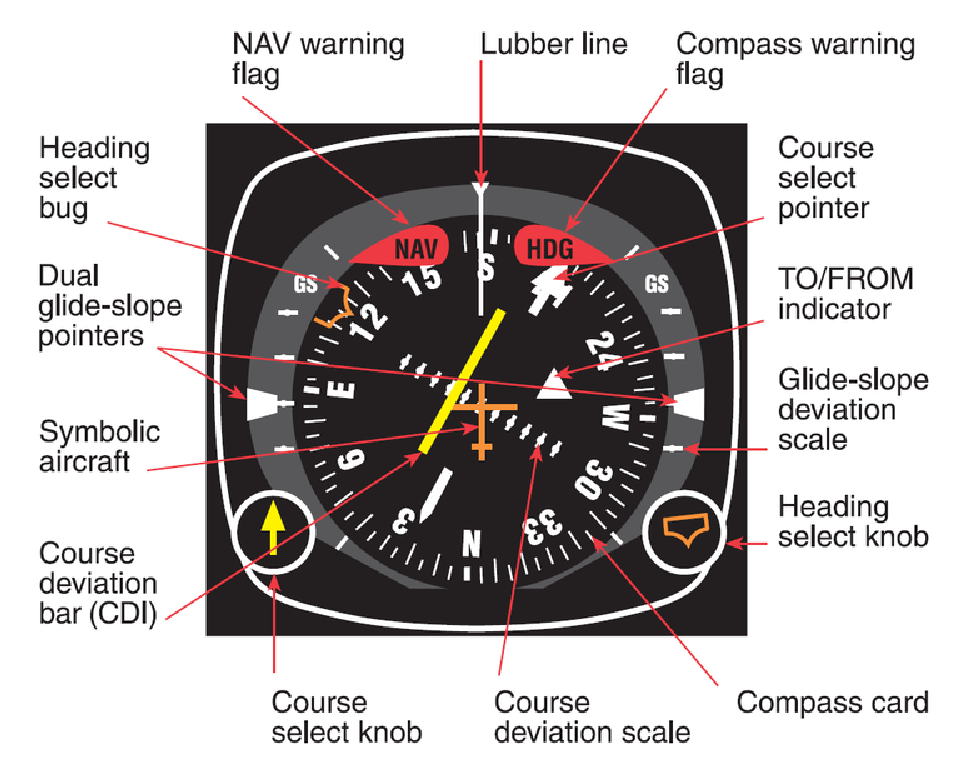
\includegraphics[keepaspectratio,width=0.7\textwidth]{06.radionavegacion/Imagenes/06.02.vor.imagenes/Wiki-HSI.eps}
  \caption{Partes de un HSI (gentileza Federal Aviation Administration )}
  \label{fig:HSI-partes}
\end{figure}

Los elementos que componen el HSI son:

\subsubsection{Rosa de rumbos (compass card) }

Actúa de la misma forma que el girodireccional del avión y está sincronizada con el sistema de brújula giroestabilizada del mismo. Bajo el índice superior del instrumento, se leerá siempre el rumbo magnético que lleve la aeronave. Las divisiones de la rosa son las mismas que las descritas para los indicadores de ADF.

\subsubsection{CDI  (Course Deviation Indicator, Indicador Desviación de Curso)}

La situación del avión con respecto a cualquier ruta seleccionada, se muestra gráficamente, pues, el CDI es totalmente móvil, pudiendo adoptar cualquier posición.

A ambos extremos del CDI están los indicadores de ruta selectada y de ruta recíproca. El primero de ellos tiene 1a forma de una pequeña espada e indica siempre la ruta seleccionada. El segundo indicador es el de ruta recíproca.

El selector de rutas OBS, es el mando situado en la parte inferior izquierda, en la Figura anterior, de la caja dell instrumento. Mediante una serie de transmisiones mecánicas hace girar a los indicadores de ruta selectada y recíproca. Naturalmente, a l ser girado el OBS. eI CDI también variara su posición en el interior del instrumento.

\subsubsection{Indicador TO-FROM}

Un sencillo triángulo situado en el centro del instrumento indica si se está volando en TO o en FROM.

Cuando el triángulo está al mismo lado que la espada indicadora de ruta selectada el avión vuela en TO. Por el contrario, si el triángulo apareciera al lado en el que está el indicador de ruta recíproca, se estaría volando en FROM.

\subsubsection{Puntos de referencia}

\begin{enumerate}

\item Existen ocho puntos de referencia situados cada 45 grados alrededor de la rosa de rumbos.

\item Un triángulo invertido en la parte superior de la caja del instrumento y un pequeño segmento en la parte inferior, constituyen las referencias de rumbo magnético y su recíproco, que lleva el avión.

\item Cinco puntos en el centro del instrumento indican el desplazamiento en grados del CDI. El valor en grados de cada punto es el mismo que en el instrumento VOR convencional. Cuando el HSI actúa como indicador de ILS, el valor de cada punto se reduce de la misma manera que en el indicador ILS clásico. 

\item También en el centro del instrumento va dibujado un pequeño avión que indica la posición relativa de éste con respecto a la ruta selectada.

\item Con eI mando instalado en la parte inferior derecha del HSI (Figura \ref{fig:HSI-partes}, Heading select knob), se hace girar la referencia situada sobre la rosa de rumbos. EI dibujo que lleva rotulado este mando tiene la misma forma que Ia referencia móvil. Esta es usada por el piloto como recordatorio de cualquier ruta o rumbo, aunque en realidad es un selector de rumbos para que el piloto automático (AUTO PILOT) inicie su seguimiento.

\end{enumerate}

\subsubsection{Indicaci\'on de senda de planeo}

En ambos lados del HSI va colocado el GSI (Glide Slope Indicator, Indicador de Senda de Planeo), mediante punteros que señalan la senda de planeo (dual glide-slope pointers).

El GSI entra en funcionamiento cuando el instrumento actúa como indicador de ILS (Instrument Landing System, Sistema de Aterrizaje por Instrumentos).

Un par de pequeños triángulos se desplazarán por encima o por debajo de un fiel indicando la posición del avión con relación a la senda de planeo de una instalación ILS. Los puntos blancos indican el desplazamiento en grados del GSI. 

Otros tipos de HSI tienen una distribución distinta de los elementos descriptos, pero básicamente son los mismos.

\begin{minipage}[c]{0.45\textwidth}
  \begin{center}
  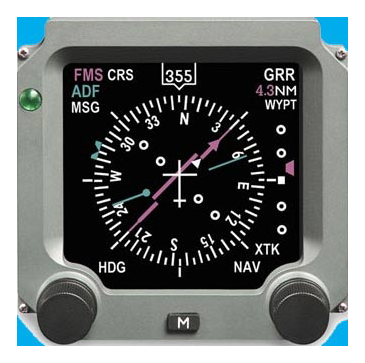
\includegraphics[width=0.9\linewidth]{06.radionavegacion/Imagenes/06.02.vor.imagenes/hsi_ehsi-4000.eps}
  \captionof{figure}{EHSI-4000 \\(Gentileza      L-3 Avionics Systems)  }
  \label{fig:HSI_001}  
\end{center}
\end{minipage}\hspace{0.05\textwidth}
\begin{minipage}[c]{0.45\textwidth}
  \begin{center}
  
\includegraphics[width=0.9\linewidth]{06.radionavegacion/Imagenes/06.02.vor.imagenes/hsi-Bendix-King-KI-825.eps}
  \captionof{figure}{HSI Bendix/King KI-825 \\(Gentileza Bendix)}
  \label{fig:HSI_002}    
\end{center}
\end{minipage}

% \begin{figure}[!h]
%   \centering
%   \subfigure[EHSI-4000 (Gentileza      L-3 Avionics Systems   )]{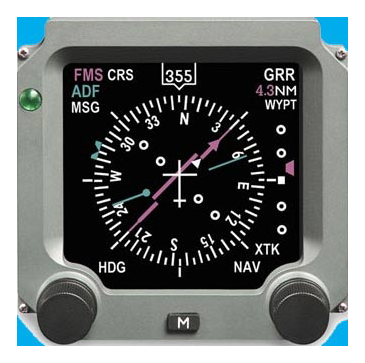
\includegraphics[width=0.45\textwidth]{06.radionavegacion/Imagenes/06.02.vor.imagenes/hsi_ehsi-4000.eps}}
% \subfigure[HSI Bendix/King KI-825 (Gentileza Bendix)]{
\includegraphics[width=0.45\textwidth]{06.radionavegacion/Imagenes/06.02.vor.imagenes/hsi-Bendix-King-KI-825.eps}}
%   \caption{Tipos de HSI}
% \end{figure}



En las Figuras anteriores pueden apreciarse HSI con pantalla de tipo Active Matrix Liquid Crystal Display (AMLCD), que resulta visible tanto con luz solar directa como en una cabina a oscuras.

\begin{enumerate}

\item En una de las esquinas va instalado el indicador del equipo radiotelemétrico (DME) dando información constante de la distancia que separa al avión de la estación selectada.


\item En una ventanilla aparece la ruta selectada mediante el OBS. 


\item Por último, en este HSI pueden verse dos referencias más, en distinto color que no son más que la cabeza y la cola de una aguja indicadora de ADF. Al ser Ia carta de HSI móvil, esta aguja trabajará como si el instrumento fuera un RMI.

\end{enumerate}



